% Generado por sistema/backend ReporteTex.java -- no editar a mano.
% Datos: CSV importado (titulados) / CSV importado (empleadores)
\textit{Paso 1. Variables.} Sobre todos los titulados que respondieron, se cruzan dos variables cualitativas -- $X$ = género, $Y$ = situación laboral -- con una variable cuantitativa -- $Z$ = años de vida profesional --, siguiendo la tabulación cruzada multivariada de la asignatura: frecuencia ($n$) y promedio de $Z$ ($\bar{Z}$) en cada combinación $X$--$Y$ que aparece en los datos.

\textit{Paso 2. Tabulación cruzada de frecuencias y antigüedad promedio.}

\begin{mitabla}{Género ($X$) y situación laboral ($Y$), con antigüedad promedio ($n=145$)}
\begin{tabular}{llcc}
\toprule
$X$ (género) & $Y$ (situación laboral) & $n$ & $\bar{Z}$ (años) \\
\midrule
Hombre & Trabaja en una organización & 85 & 9.39 \\
Mujer & Trabaja en una organización & 22 & 9.50 \\
Hombre & No trabaja & 16 & 4.31 \\
Hombre & Emprendimiento propio & 12 & 9.92 \\
Mujer & No trabaja & 8 & 7.88 \\
Mujer & Emprendimiento propio & 2 & 11.00 \\
\midrule
\multicolumn{2}{l}{Total / Promedio general} & 145 & 8.83 \\
\bottomrule
\end{tabular}
\end{mitabla}

\begin{figure}[H]
\centering
\caption{Promedio de antigüedad promedio por combinación $X$--$Y$ (años)}
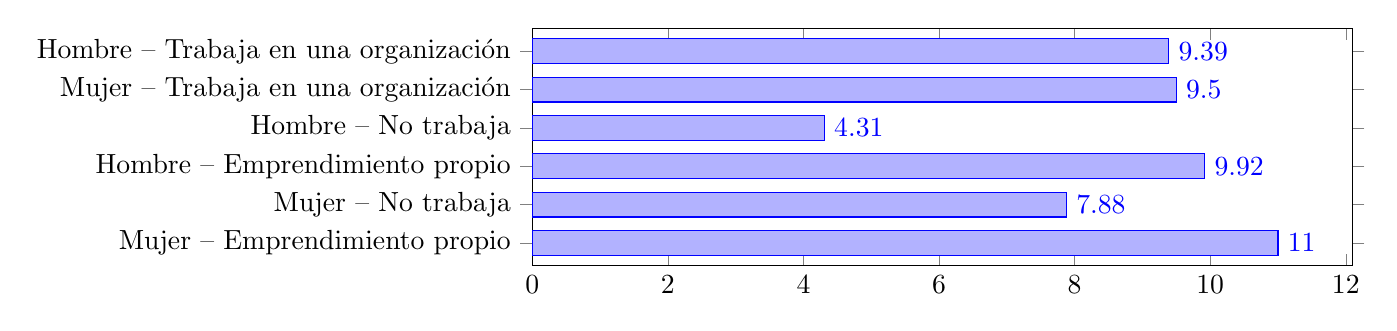
\begin{tikzpicture}
\begin{axis}[
  xbar, bar width=9pt,
  width=12cm, height=4.6cm,
  xmin=0,
  ytick={0,...,5},
  yticklabels={Hombre -- Trabaja en una organización,Mujer -- Trabaja en una organización,Hombre -- No trabaja,Hombre -- Emprendimiento propio,Mujer -- No trabaja,Mujer -- Emprendimiento propio},
  ymin=-0.6, ymax=5.6,
  nodes near coords, y dir=reverse,
  every axis plot/.style={fill=gray!60}
]
\addplot coordinates {(9.39,0) (9.50,1) (4.31,2) (9.92,3) (7.88,4) (11.00,5) };
\end{axis}
\end{tikzpicture}
\end{figure}

\textit{Paso 3. Hallazgos por categoría de $X$.} Para cada categoría de género, la categoría de situación laboral más frecuente y si antigüedad promedio queda por encima o por debajo del promedio general (8.83 años):

\begin{itemize}
  \item \textbf{Mujer} ($n=32$): Antigüedad promedio de 9.19 años, por encima del promedio general. La categoría de situación laboral más frecuente es trabaja en una organización (68.8\% de este grupo).
  \item \textbf{Hombre} ($n=113$): Antigüedad promedio de 8.73 años, por debajo del promedio general. La categoría de situación laboral más frecuente es trabaja en una organización (75.2\% de este grupo).
\end{itemize}

\textit{Interpretación.} La antigüedad promedio varía más por la situación laboral que por el género dentro de cada grupo: quienes están en un emprendimiento propio o no trabajan tienden a mostrar promedios distintos a quienes trabajan en una organización, independientemente del género. Esto es exploración descriptiva, no una prueba de independencia.

